\documentclass[12pt,a4paper]{article} 
\usepackage[portuguese]{babel}
\usepackage[utf8]{inputenc}
\usepackage{adjustbox}
\usepackage{amsmath}
\usepackage{graphicx}
\usepackage{booktabs}
\begin{document}
\setcounter{figure}{3}
\setcounter{section}{3}
\setcounter{page}{7}
\section{Relatório}
\subsection{Introdução}
Pretende-se neste prática enteder o comportamento do diodo em diferentes circuitos . Para tal finalidade, montou-se um circuito retificador, um circuito ceifador e um circuito limitador alimentados com alimentação \emph{AC}.
.

\subsection{Análise}
Montou-se o circuito retificador de meia onda, representado pela Figura~\ref{fig:circ_retif}, alimentado por uma tensão senoidal,    produzido por um gerador de ondas, de 100$Hz$ para três valores de  picos de tensão diferentes, $500mV$, $5V$ e $10V$. 
Com a ajuda de um ociloscópio, analisou-se o sinal de entrada, saída, o valor médio e a tensão de pico de cada circuito em diferentes condições, estes dados estão presentes na Tabela~1. Também obteu-se dados da tensão de entrada e de saída, que originaram os gráficos da Figura~\ref{fig:retifi}--\ref{fig:retificador10}.
\begin{figure}[htpb]
  \centering
  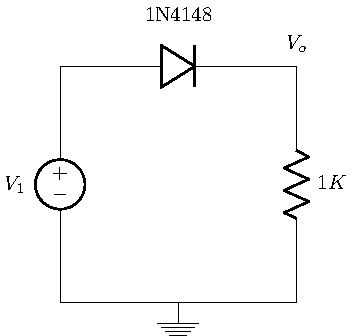
\includegraphics{./circ_retif.pdf}
  \caption{Circuito retificador montado para o experimento número 1.}
  \label{fig:circ_retif}
\end{figure}
\begin{figure}[htpb]
  \centering
  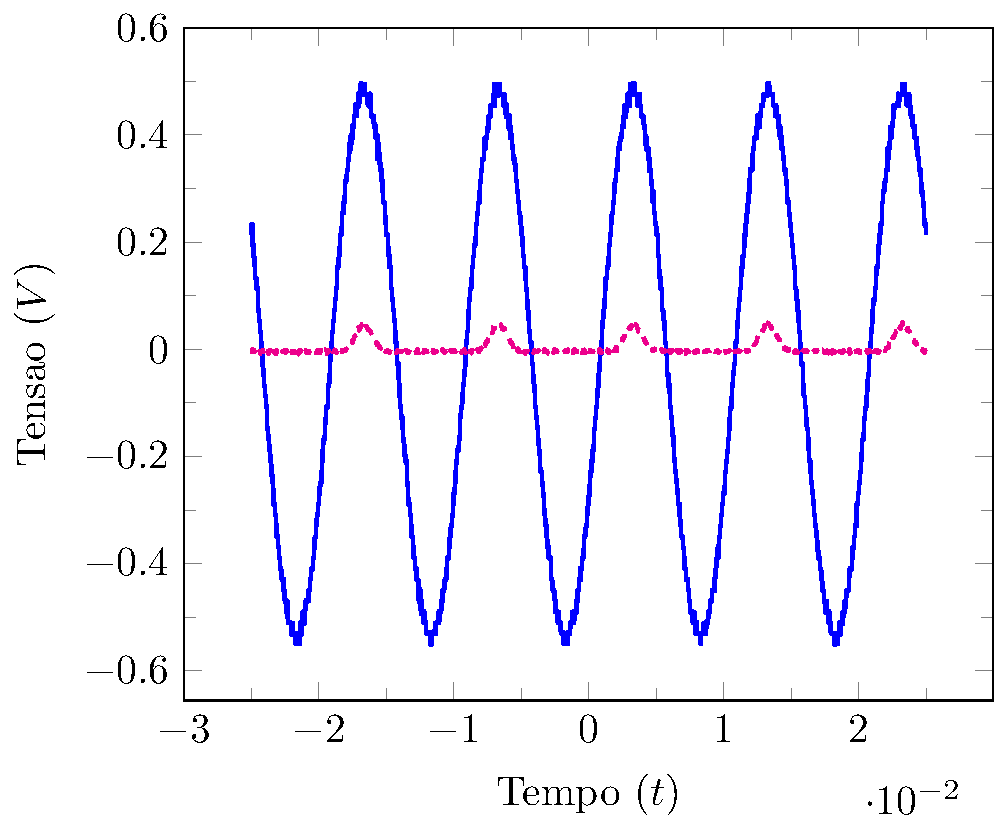
\includegraphics[width=0.8\linewidth]{./retificador_meio.pdf}
  \caption{Circuito retificador de meia onda para uma tensão de pico de $V_1=500mV$. A linha em azul, contínua, representa o sinal de entrada, enquanto a linha pontilhada em magenta representa o sinal de saída.}
  \label{fig:retifi}
\end{figure}
\begin{figure}[htpb]
\centering
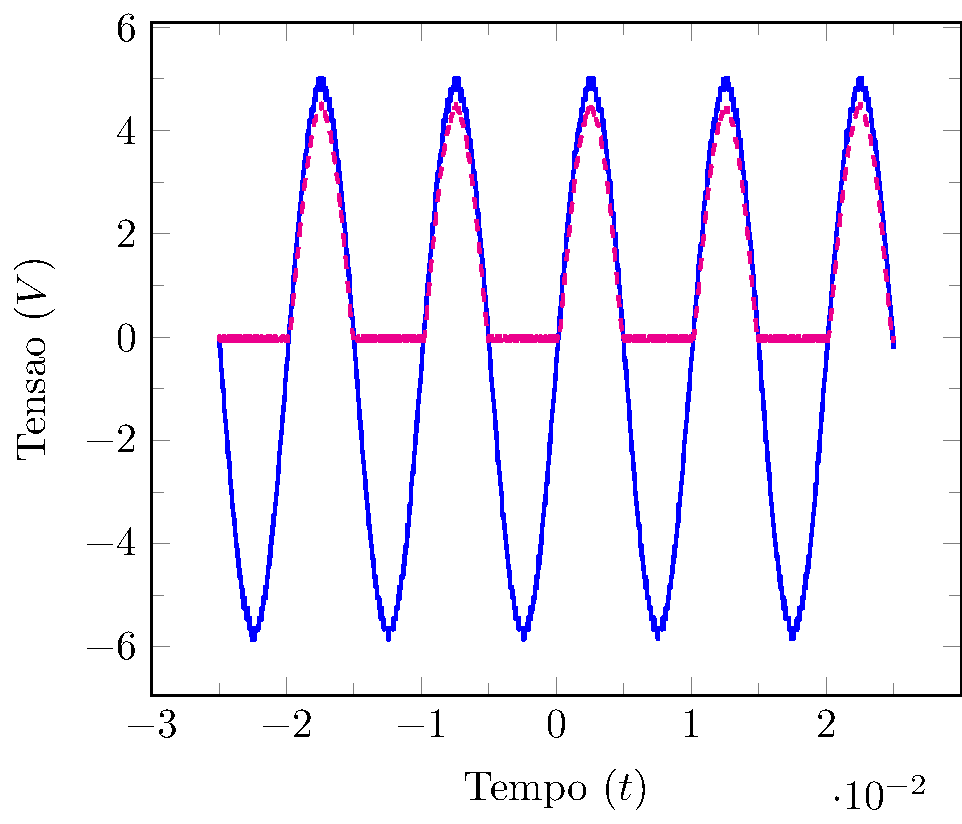
\includegraphics[width=0.8\linewidth]{./retificador_5.pdf}
  \caption{Circuito retificador de meia onda para uma tensão de pico de $V_2=5V$. A linha em azul, contínua, representa o sinal de entrada, enquanto a linha pontilhada em magenta representa o sinal de saída.}
\label{fig:}
\end{figure}
\begin{figure}[htpb]
  \centering
  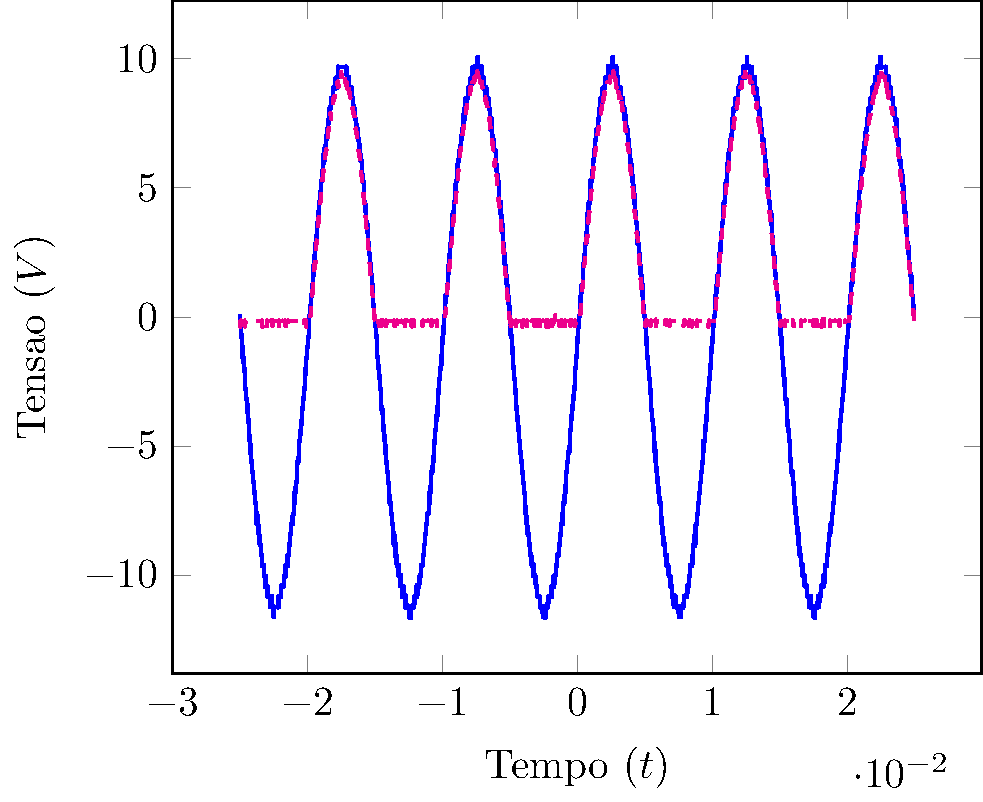
\includegraphics[width=0.8\linewidth]{./retificador_10.pdf}
  \caption{Circuito retificador de meia onda para uma tensão de pico de $V_3=10V$. A linha em azul, contínua, representa o sinal de entrada, enquanto a linha pontilhada em magenta representa o sinal de saída.}
  \label{fig:retificador10}
\end{figure}

Para o segundo experimento, montou-se um circuito ceifador, representado pela Figura~\ref{fig:circ_ceifador}. Neste experimento foi fixado no gerador de ondas uma tensão senoidal de $10V$ a $100Hz$, variando apenas a tensão contínua para os valores de $4V$ e $7V$.  Para $4V$ obteu-se uma tensão média de $-1.72V$ e de pico $5V$, e para $7V$ uma tensão média de $-853mV$ e de pico $8.2V$. Os gráficos resultantes do experimento estão representados na Figura~\ref{fig:ceifador} e Figura~\ref{fig:ceifador2}.
\begin{figure}[htpb]
  \centering
  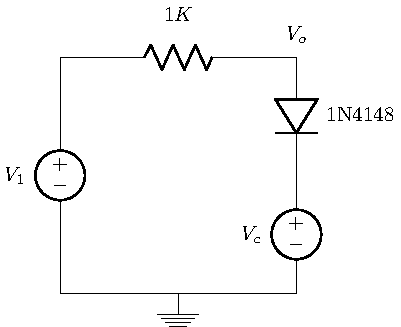
\includegraphics{circ_ceifador.pdf}
  \caption{Circuito ceifador montado para o experimento número 3.}
  \label{fig:circ_ceifador}
\end{figure}

\begin{figure}[htpb]
  \centering
  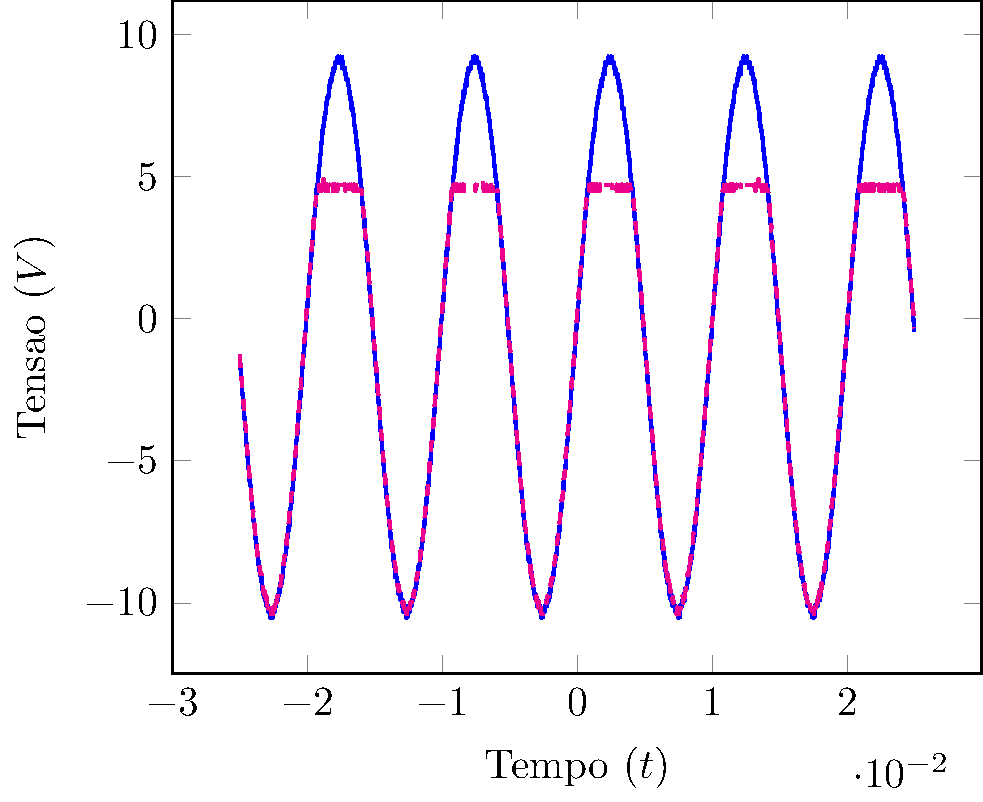
\includegraphics[width=0.8\linewidth]{./ceifador.pdf}
  \caption{Circuito ceifador para uma tensão contínua de $V_4=4V$ e tensâo de pico $V_{p}=10V$. A linha em azul, contínua, representa o sinal de entrada, enquanto a linha pontilhada em magenta representa o sinal de saída.}
  \label{fig:ceifador}
\end{figure}
\begin{figure}[htpb]
\centering
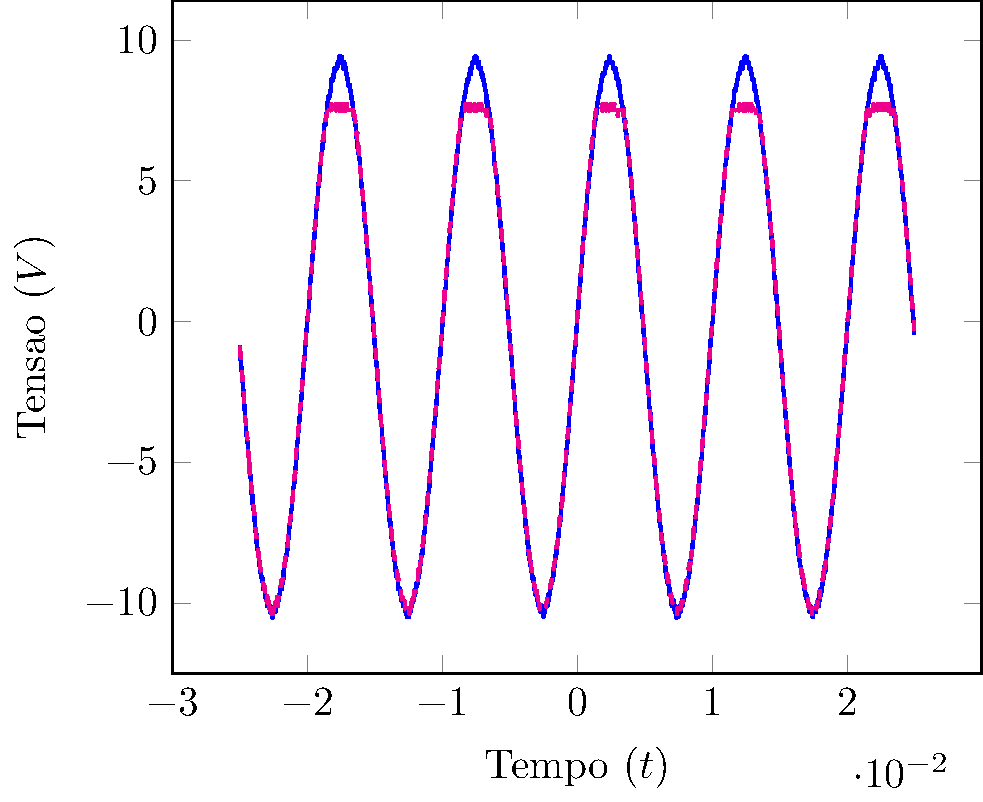
\includegraphics[width=0.8\linewidth]{./ceifador2.pdf}
\caption{Circuito ceifador para uma tensão contínua de $V_4=7V$ e de tensão de pico $V_{p}=10V$. A linha em azul, contínua, representa o sinal de entrada, enquanto a linha pontilhada em magenta representa o sinal de saída.}
\label{fig:ceifador2}
\end{figure}

O terceiro experimento baseou-se no circuito grampeador, mostrado na Figura~\ref{fig:circ_grampeador}. Com um sinal de entrada de $5V$ a $100Hz$ obteve-se uma tensão média de $9.32V$ e o gráfico da Figura~\ref{fig:grampeador}
\begin{figure}[htpb]
  \centering
  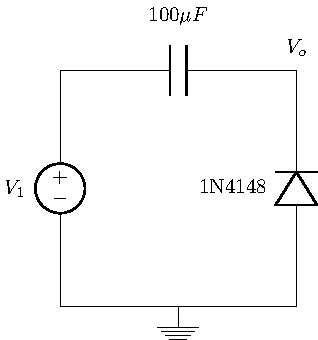
\includegraphics{circ_grampeador.pdf}
  \caption{Circuito grampeador montado para o experimento número 3.}
  \label{fig:circ_grampeador}
\end{figure}
\begin{figure}[htpb]
  \centering
  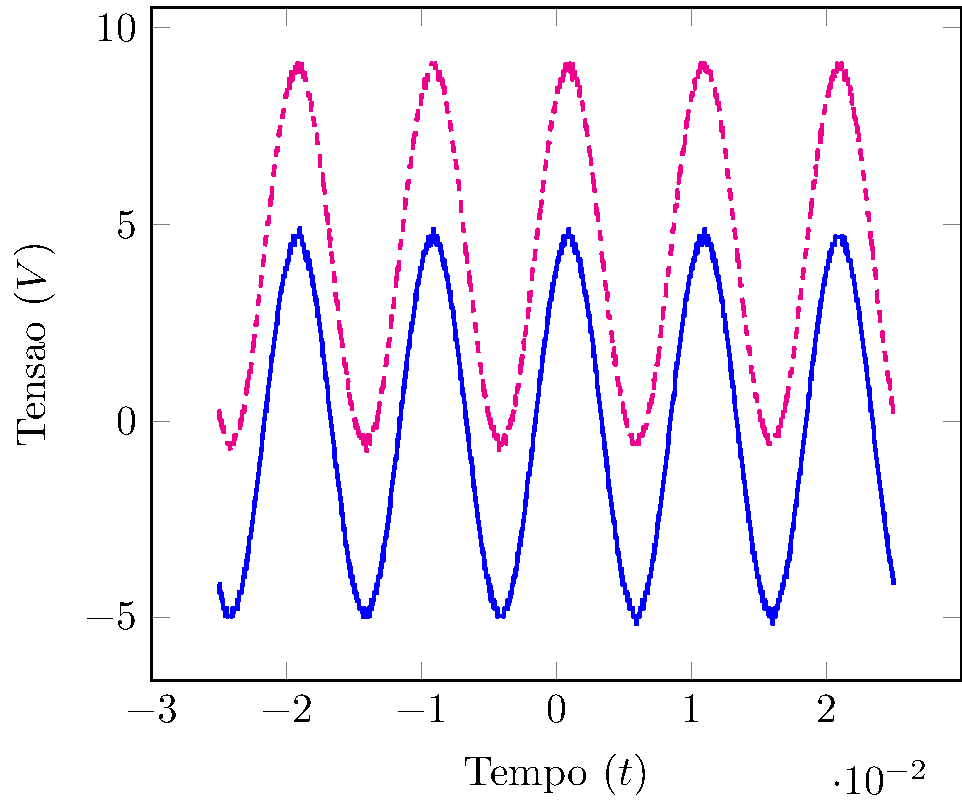
\includegraphics[width=0.8\linewidth]{./grampeador.pdf}
  \caption{Circuito grampeador para uma tensão de pico de $V_5=5V$. A linha em azul, contínua, representa o sinal de entrada, enquanto a linha pontilhada em magenta representa o sinal de saída.}
  \label{fig:grampeador}
\end{figure}
\newpage
\subsection{Discussões}
Percebeu-se o efeito do circuito retificador nas Figuras~\ref{fig:retifi}--\ref{fig:retificador10} onde apenas um ciclo de tensão senoidal aparece. Isto ocorre pois o circuito é um retificador de meia onda, ou seja, o diodo bloqueia a passagem de corrente para valores de tensão menores que $V_d=0.7V$, o que resulta apenas os semi-ciclos positivos na saída. Quando passou-se corrente, percebe-se também que, diferente de nosso modelo ideal, há queda de tensão no diodo, o que resulta em uma tensão de pico, aproxidamente, $0.7V$ menor. Existe também um pequeno atraso, antes inexistente, para a onda retificada começar a subir no semi-ciclo positivo, que corresponde aos valores entre $0V$ e $0.7V$ que ainda são pequenos demais para fazer o diodo conduzir significativamente corrente elétrica. 

Calculou-se através da fórmula, $V_{dc}=0.318V_{m}$, e da tabela 1 os valores estimados para a tensão média e o erro percentual:
\begin{align}
  V_{dc1}=0.318  \times 0.5 = 159 mV\\
  E_{1}=\frac{ |0.159-0.28 |}{ 0.159} = 76.1\% 
\end{align}
\begin{align}
  V_{dc2}=0.318  \times 5 = 1.59 V\\
  E_{2}=\frac{ |1.59-1.105 |}{ 1.59} = 30.5\% 
\end{align}
\begin{align}
  V_{dc3}=0.318  \times 10 = 3.18 V\\
  E_{3}=\frac{ |3.18-2.675 |}{ 3.18} = 15.89\% 
\end{align}
Nota-se assim, que o erro percentual diminui consideravelmente a medida que o valor da tensão de pico se torna muito maior do que a queda de tensão constante no diodo.

Ao consultarmos o datasheet do diodo 1N4148 podemos notar que seu valor máximo de voltagem de pico repetitiva é $100V$ o que o torna incapaz de ser utilizado em uma tensão de alimentação de $220V$ alternada, já o valor de pico para tal alimentação seria de $220\sqrt{2}$, muito acima dos $100V$ recomendado pela especificação.

O circuito ceifador, representado na Figura~\ref{fig:circ_ceifador}, tem como função ceifar parte do sinal aplicado em sua entrada. Observamos nas Figuras~\ref{fig:ceifador}--\ref{fig:ceifador2}, que parte do semi-ciclo positivo foi limitado por um valor proporcional ao valor da  fonte $V_{c}$ constante. O valor em que a tensão será ceifada é dada por:
\begin{align}
  V_{limit}= V_{1}+V_{d}
\end{align}
Onde $V_{limit}$ é o valor em que a tensão é ceifada, $V_{1}$ é o valor da fonte de tensão constante e $V_{d}$ é a queda de tensão de um diodo dado que ele está conduzindo.

O circuito grampeador, representado na Figura~\ref{fig:circ_grampeador}, tem como função elevar ou abaixar a entrada através da mudança de seu nível DC. O circuito é composto de um capacitor, que armazena carga DC, e de um  diodo que serve para conduzir corrente em apenas um sentido, impedindo que o sinal de exceder seu valor de referência. A relação entre a tensão de pico de entrada e de saída é $V_o=V_{capacitor}+V_{pico}+V_1$, como observado na Figura~\ref{fig:grampeador}.
\newpage
\subsection{Conclusão}
Ao apresentar e elucidar os conceitos sobre as diversas possíveis aplicações de diodos em circuitos elétricos, concluí-se que a prática foi de imenso proveito. O circuito retificador foi ilustrado com detalhes, para diversos sinais de entrada e pode-se aferir o quão bom é a aproximação de sua tensão média, dado o valor de pico do sinal de entrada. 

Os circuitos grampeador e ceifador,  até então desconhecidos pela dupla, foram apresentados e compreendidos como ferramentas fundamentais para se projetar circuitos elétricos. O ceifador pareceu ser ideal para proteger cargas de tensões indesejadas e o grampeador, no caso, agiu como um filtro para evitar tensões negativas (ou positivas).
\end{document}
